\section{Company information}

\subsection{Organization}
When we talk about company information, we focus our interest on the points
that can give us a detailed view of the entire business and its processes. This
type of essential information is usually found on the target company's
websites. We will not necessarily find all the necessary information to give us
an {\bf insight} into the company and its {\bf processes}. This could tell us which
companies will be most interested in working with our target company and which
requirements must be met. Understanding our target company's business processes
can give us an idea of how to structure our attacks. Therefore we can design
our attacks to be executed during a specific step in the process.

We can also get an insight into the company's dependencies. From this, we will
be able to conclude which technologies are needed to manage the company, which
will indicate how the company may be structured from an infrastructure
perspective.
\begin{figure}
  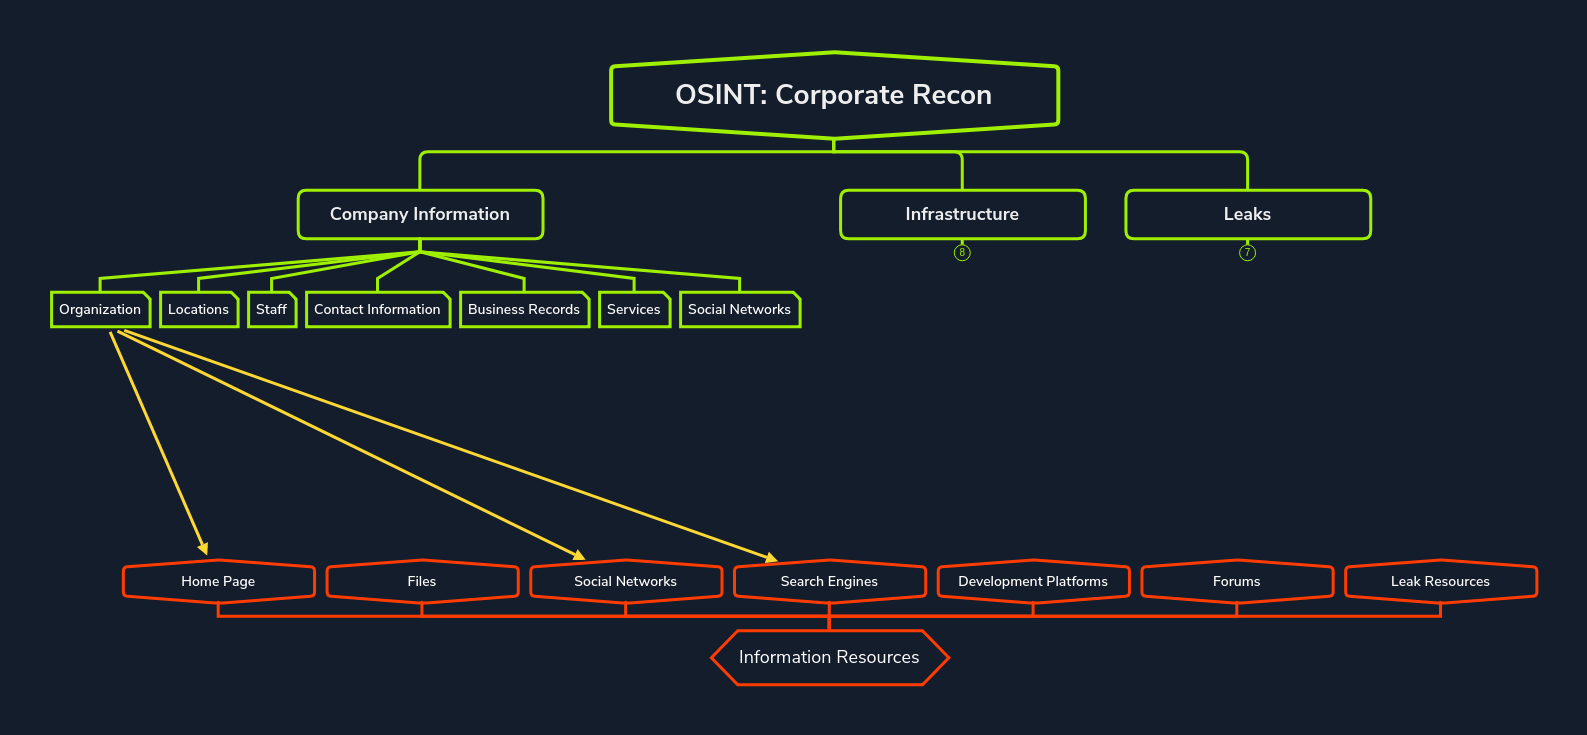
\includegraphics[width=\linewidth]{recon/osint/images/osint-org.png}
  \caption{OSINT Organization}
  \label{fig:osint-org}
\end{figure}

Generally, the company's home page, social networks, and search engines can be
used to map out the company's organizational structure. There are no useful
tools that can be used to map out the company's organizational structure
efficiently. Instead, we must rely on the logical association between the
information we will find during OSINT and the actual intelligence.

Furthermore, it is challenging to keep it dynamic because every company has
unique staffing needs and employees, all of whom bring different strengths,
weaknesses, and abilities. Therefore this field of OSINT is more a repeatable
process than a static method.

\subsection{Locations}
If our engagement is a red team assessment, then such information is much more
relevant than a regular penetration test procedure. Red-teaming can also
include, among other things, the physical security of the company and is used
to determine which methods and techniques can be used to obtain highly
sensitive information that may not be accessible from the internet. The
company's locations are of great importance for this. However, the scope and
rules for which procedures may and may not be used must be strictly observed.

Companies already pay a lot of money to attract potential customers by
presenting themselves to their customers in the best possible way and sell
themselves better from a marketing point of view. Here we can always ask
ourselves when the company would arouse our {\bf interest}.

\begin{figure}
  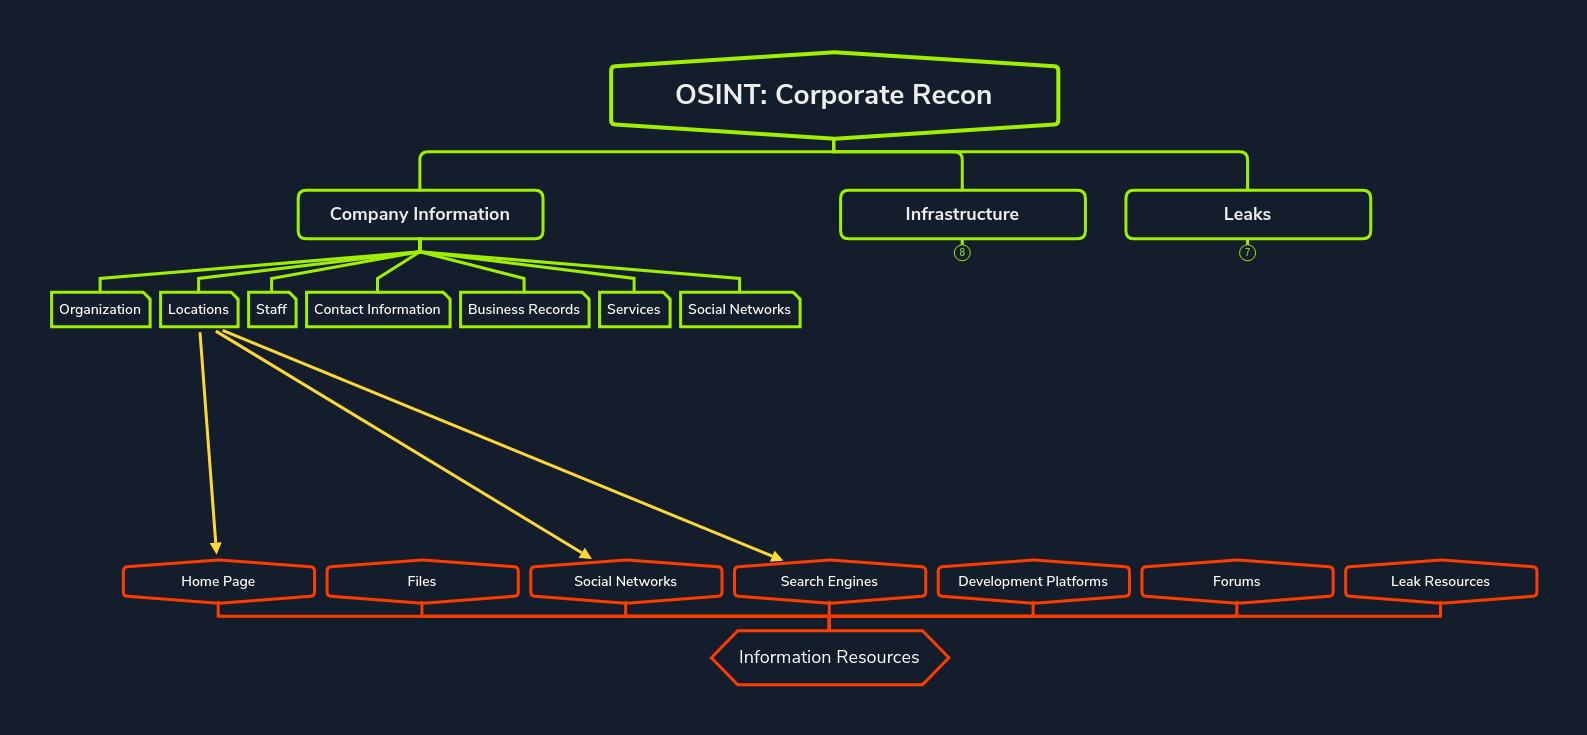
\includegraphics[width=\linewidth]{recon/osint/images/osint-locations.png}
  \caption{OSINT Locations}
  \label{fig:osint-locations}
\end{figure}

When we look into a company's locations, we have to identify the most obvious
locations in advance. Larger companies that are active in the field of
production sometimes have sites that they do not mention. These can also be
identified in the OSINT process. The most prominent locations are usually
listed on the company's home page. After all, the company wants to attract
potential customers with the number of locations it has. It is an overall
strategy for companies to present themselves as the best all over the world.
This contributes significantly to marketing and increases the number of
customers and thus the turnover.

In general, we can find basic information about a company's locations in
advance using the following resources

\subsubsection{Home Page}
If we start with the home page and browse through the site a little, we will
find {\bf countries}, {\bf cities}, {\bf addresses}, and possibly even maps
that show the company's locations. 

Most of the time, we will also find lists that include the countries and/or
cities where the company has its offices. These locations are usually managed
locally by administrators but also may be managed centrally. If the company is
centrally managed, these locations (either the entire company or specific
locations) within the scope can also provide us with attack vectors that we can
use to get into the systems' central administration infrastructure.

\subsubsection{Social Networks}

Social networks are used to share much information, especially information that
potential customers can use to learn more about the company. This includes the
publication of locations of offices or production facilities. This type of
information can be found on many social networks such as Twitter, LinkedIn,
Instagram, Snapchat, YouTube, WeChat, Facebook, and others. Most links to a
company's social networks can be found on their home page.

\subsubsection{Search Engines}

Every company location can provide us with another potential attack vector,
whether physical or technical. Each site has different employees and managers
who have their way of working and can open up different attack paths for us
than other locations. As soon as we have detailed information about the
locations, we should document them and, in the best case, add a graphical
representation as evidence in our documentation. For example, we can use
\href{https://maps.google.com/}{Google Maps},
\href{https://earth.google.com/web/}{Google Earth},
\href{https://showmystreet.com/}{ShowMyStreet}, and many others to obtain these
types of views.

In this case, we could pretend to be a significant client for potential
collaboration and organize a meeting to be let into the building and get a much
better insight into the company's processes. If the contract requires a
physical test, we can also get an inside view of the building's physical
security, such as door locks, windows, security, cameras, rooms, departments,
and more.

Information about locations is mainly interesting for {\bf physical Red Team}
operations. This is because it distinguishes between the times at which a
"break-in" can be most efficient. If a physical assessment is conducted during
working hours, we must be granted appropriate access to restricted areas
upfront. If possible, it is better to find a way to enter the building at night
if the alarm systems and their vulnerabilities allow it. The locations
themselves are the company's buildings and the location of the offices.
Sometimes there are also badge readers that we can see and use to identify how
to set up our cloner to hijack access cards wirelessly.

Suppose a manager or even higher employee feels safe in their office, which has
only access to a minimal number of employees and suddenly finds a USB stick on
their desk. In that case, they may wonder where it came from. The feeling of
being safe increases the likelihood that the USB stick we leave behind will be
plugged into their computer.

In larger companies, we will find some of these locations, which at first
glance already indicate some potential weaknesses in the field of physical
security. Suppose we have such an assignment where we also have to test the
organization's physical security. In that case, we can use the same resources
to get a picture of the terrain or even physically walk through the location as
a "passerby" and record a video of the terrain with a simulated phone call.
Depending on whether the location and the terrain allow it, we can also take
photos from a distance. By using the online resources, we will also be able to
gain some information.

We have to keep in mind that these photos have not been made today and may not
be up to date. Nevertheless, if we take a closer look at them, we can see some
interesting characteristics of the building, which could be helpful for us.


\subsection{Staff}
Every company's marketing department attaches great importance to the best
possible representation of its {\bf staff} so that potential customers can be
sure they will be taken care of in a professional manner. The company's
employees handle all the processes. We are interested in the information they
use to interact with the company and its infrastructure. This may include but
is not limited to email addresses, phone numbers, usernames, passwords, and the
social networks on which they operate.

The employee's role in the company can also be used to assess their privileges
in specific areas. Thus, a manager would likely have higher rights than
customer support. However, even if a secretary does not have direct access to
the systems, the individuals in these roles can be an attractive attack vector
for us since they most likely have full access to calendars, plans, contact
data, email addresses, and more.

\begin{figure}
  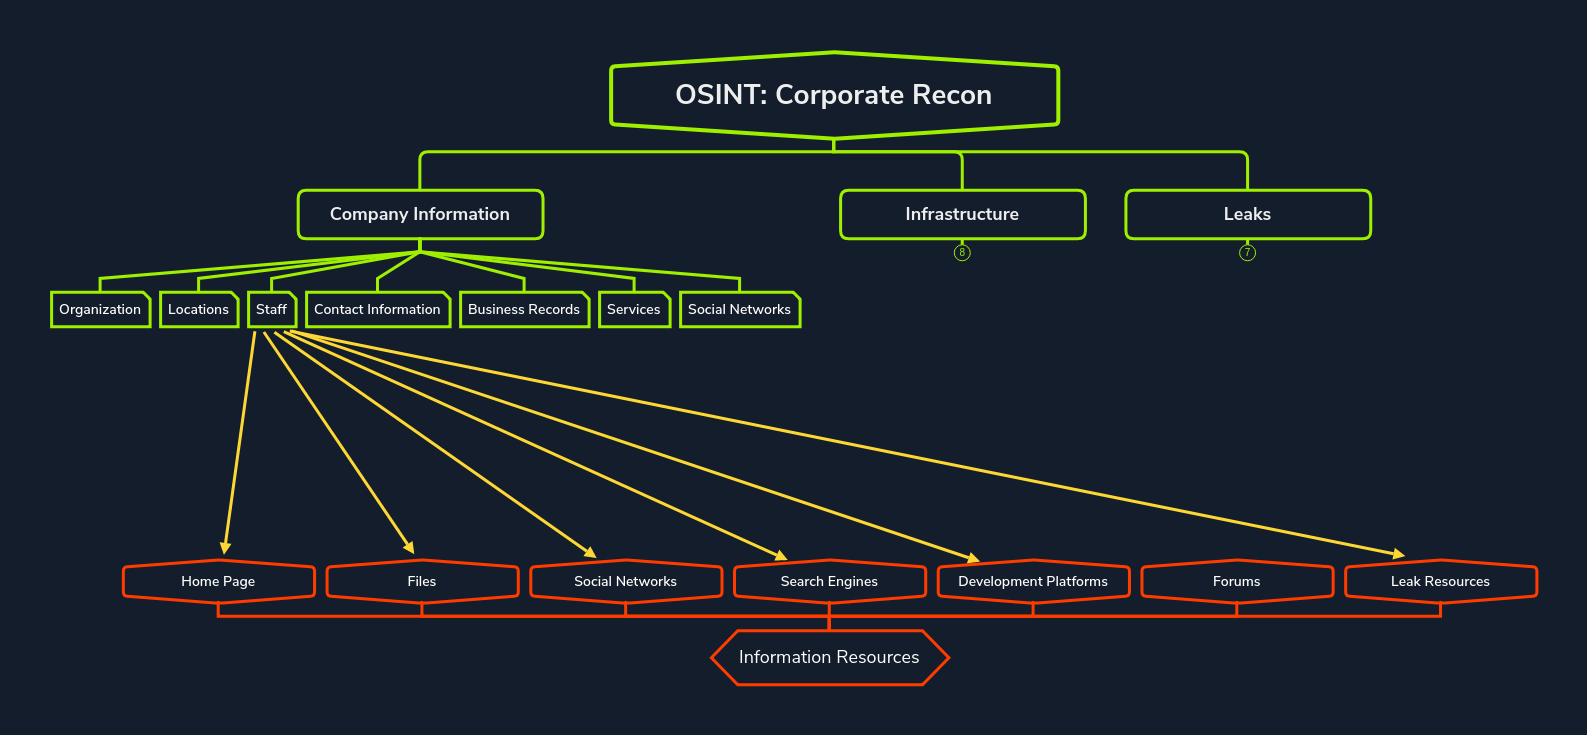
\includegraphics[width=\linewidth]{recon/osint/images/osint-staff.png}
  \caption{OSINT Staff}
  \label{fig:osint-staff}
\end{figure}

Information about the company's employees and managers is essential for us,
enabling us to reconstruct the internal corporate structure. With this
information, we will be able to identify the different departments' managers
and design our social engineering attacks better and more efficiently. We are
not yet looking at individual employees, but rather looking at who is employed,
who is in charge of what, who is responsible for what, and try to get a picture
of the internal communication flow.

The methodology we have used so far can also be applied to staff. However, this
field covers many potential attack vectors for {\bf phishing campaigns} and
{\bf social engineering} attacks, which we need to filter out. We will get many
valuable results, but this does not cover everything applied to the staff. This
field will be discussed in more detail in the Module {\bf OSINT: Staff
Investigation}.

In this step, we should continue to focus on getting an overview of the
company's employees to gain insight into its internal structure and hierarchy
and to be able to reconstruct it if necessary.

There are many sources we can use to obtain this information. Among them are
the following

\subsubsection{Home Page}
Most of the time, we can find the company's essential contact persons on the
"About Us" page. These staff members are usually trained to present themselves
professionally to customers and have the necessary answers to the most critical
questions.

It is interesting to note that we can read a biography for the C-level staff
here. This can serve us very well later in social engineering to find common
topics we can discuss and gain a certain amount of trust and sympathy from the
relevant persons. An important thing to note here is that these people would
only deal with large customers who promise a significant profit. Otherwise, it
can be hard to get directly to them.

We are interested in the employees who are already employed and want to know
what types of employees the company is actively recruiting. IT offers many
different specializations, enabling us to identify which technologies the
company works with or plans to work with by reading through open job
requisitions. Therefore we can continue to search for job offers on the
homepage that are still open or on the company's LinkedIn profile.

\subsubsection{Files}
Often companies offer different flyers, reports, and news in the form of files.
The software used to create these files is usually registered and only
available to authorized employees registered in the system. This data also
includes the software that labels the created files with metadata. These can
then be extracted and read out with the help of exiftool~\ref{tool:exiftool} or
metagoofil. This
information can include usernames, dates, software and version numbers,
geographical coordinates, and much more. We should download as many accessible
files as possible and extract the metadata accordingly.

\subsubsection{Social networks}
Finally, most employees do not want to miss the opportunity to get better job
offers from other companies and keep their profiles updated on business
networks. Maybe even with the latest projects they had to deal with to show off
their skills. Every company wants to have the best possible presence on social
media and, therefore, publishes links to their company profiles. These are
often also linked to the profiles of all their employees. One such source could
be LinkedIn, for example.

Apart from the individual employees and their profiles, LinkedIn can also give
us a better overview of our target company. For example, we can find out an
estimated number of employees for our target company.

On LinkedIn, we can also enter specific keywords in the search field, which
will filter the target company employees to make our search more specific. We
need people who work on computers and typically are not interested in those
that do not use a computer at all in their day-to-day jobs.

inally, we have filtered out our potential targets very well and have specific
ones to focus our attention. All business and social networks will be covered
in a later section. Other valuable sources for employees and job positions
are:
\begin{verbatim}
Xing 	
Monster 	
Indeed 	
Glassdoor 	
TrustPilot
\end{verbatim}

iFurthermore, we can use {\bf search engines} we know from which we will
discover other employees, the social networks on which they appear, the {\bf
development platforms} used by developers, and other files from which we can
extract metadata. We can obtain further information through these {\bf internal
leaks}. The search for employees requires an adapted approach and represents an
additional larger field of information sources. It is crucial to examine them
separately. Otherwise, we might get stuck in this phase. This will become much
clearer in the {\bf OSINT: Staff Investigation Module}.


\subsection{Contact Information}
Another critical point for all potential customers is the company's
accessibility. For this reason, {\bf contact details} are always disclosed.
After all, customers may want to find out more about the company or even
arrange a meeting. Contact information includes phone numbers and email
addresses, and usernames from various communication portals such as Skype,
Microsoft Teams, Slack, Discord, etc. These usernames can also be associated
with the employees. This part of OSINT will be discussed in more detail at {\bf
OSINT: Staff Investigation}.

\begin{figure}
  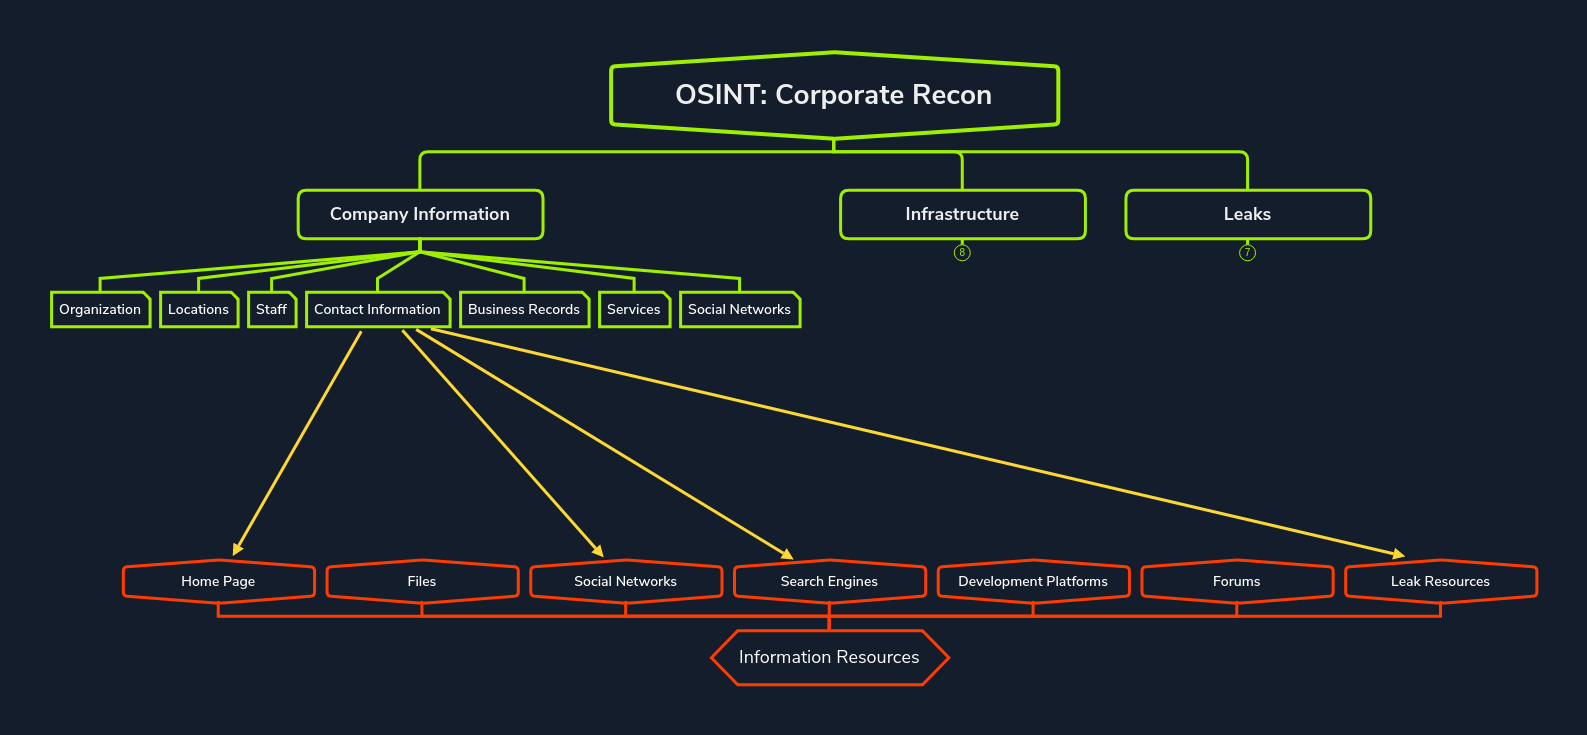
\includegraphics[width=\linewidth]{recon/osint/images/osint-contact.png}
  \caption{OSINT Contact}
  \label{fig:osint-contact}
\end{figure}
Contact details may be relevant to contact the appropriate person and send
inquiries to find out more about the company's processes. These may include
technical issues where we want to ensure that the products we offer will work
with our working environment.

\subsubsection{Home Page}
For example, in the next Penetration Testing phase, we could call the {\bf
phone numbers} to pretend to be customers of the company, ask short technical
questions, and ask them to help us with our issues. It is also interesting to
note that larger companies often have more than one domain. Therefore, the
contact persons' {\bf email addresses} may be on a different domain than the
one on which the main website is located. We could, for example, use these to
prepare our phishing campaigns and use these email addresses as targets.
Phishing attacks can provide us with sensitive information, such as passwords
or usernames, which can be very helpful, if not essential, in our penetration
testing process.

This information is crucial for us, especially for phishing, vishing, and
social engineering attacks in the {\bf Exploitation phase}. Employees from the
customer service and sales teams communicate a lot with (potential) customers
and therefore easily fall into a routine requiring repetitive processes. By
human nature, routine operations reduce the attention span, leading to the
inattentive and careless performance of their tasks. This is one of the
weaknesses that we can use for our purposes when we talk to an employee and
influence them to click on a link we send him.

\subsubsection{Social Networks}

Social networks provide us with a platform for interacting with the company's
employees and offer a wide variety of information about them. It is irrelevant
whether these are private social networks or business networks. What is
important is that we can obtain additional information through each of these
networks, including {\bf contacts}, {\bf partners}, {\bf co-developers}, their
{\bf phone numbers}, and {\bf email addresses}.

\subsubsection{Search Engines}

It is also beneficial to note down all the persons' {\bf names} because they have to log in to their domain with the respective identifiers or unique name format. IT people are especially interesting because most companies allow IT people to do their work from home. This indicates that there must be a specific type of remote access mechanism for connecting to the internal network remotely.

Another excellent source to find out the email addresses of the target domain
is \href{https://www.hunter.io/}{Hunter.io}.

We can verify each email address via \href{https://emailrep.io/}{Emailrep.io} and check how the mail servers handle it.
\begin{verbatim}
curl emailrep.io/<firstname>.<lastname>@<domain>.<tld>
\end{verbatim}

\href{https://rocketreach.co/}{RocketReach} allows us to identify email address formats by domain and the other email addresses linked to the corresponding managers. It is a paid service provider, but the results we get from it are very accurate, and it is an excellent way to find out links to the company's employees and the platforms they use.


\subsubsection{Leak Resources}

When we talk about leaks, we are not just talking about published databases
that contain users' passwords and email addresses. Apart from the fact that
these databases offer an excellent research opportunity, if we know the domain
to which the email addresses are registered, we can also find new and unknown
email addresses.

Apart from that, \href{https://web.archive.org/}{WayBackMachine from
Archive.org} offers us a very effective way to search for contact information.
It shows us older versions of the company website when IT security was less in
focus than today. Before a company becomes large, the bosses establish
themselves much more in all the necessary processes to efficiently control
them. Therefore, email addresses were often published on the websites at that
time to establish contact with the managers and customers better. However, in
most cases, these email addresses are rarely changed by bosses and
highly-positioned members. Therefore, we need to review snapshots of the target
company website on WayBackMachine as part of the OSINT process. Below is an
example of the various snapshots taken for a sample target company. Browsing to
one of these would show us the state of the company website on the given date,
which may differ significantly from the current website version and provide us
with useful information or even expose hidden functionality.

\subsection{Business records}
Significant customers look at the company's website and the {\bf business
records}, to learn more about it. From an OSINT perspective, they can also tell
us a lot about its progress. These include the company's {\bf locations}, {\bf
financial situation}, {\bf references}, and {\bf reputation}. We are
particularly interested in poor feedback about the company.

Poor feedback requires poor communication and the resulting i{\bf failures in
the business processes}. If a customer's inquiry or request is not fulfilled,
it may not always be a human mistake on the part of the employee but may
indicate technical issues. Companies often try to "hide" this feedback not to
create a wrong impression for potential customers.

Business records also include the degree of recognition in the market. For
example, we can get this through reviews by (former) employees or on social
networks. Customer satisfaction also plays a role. We can conclude how
structured and coordinated the company works internally to complete its
services and overcome customer problems for the services provided.

The company's financial situation tells us a lot about its commitment and
productivity. If a company continually offers new products and services, it can
positively affect its financial situation. Depending on the company's size, the
downside of this is that it can lead to chaotic processes. This can mean a
great deal of organizational effort and communication. Therefore, it leads to a
higher risk of phishing attacks because the content of a detailed, customized
phishing email is rarely actually checked.

\begin{figure}
  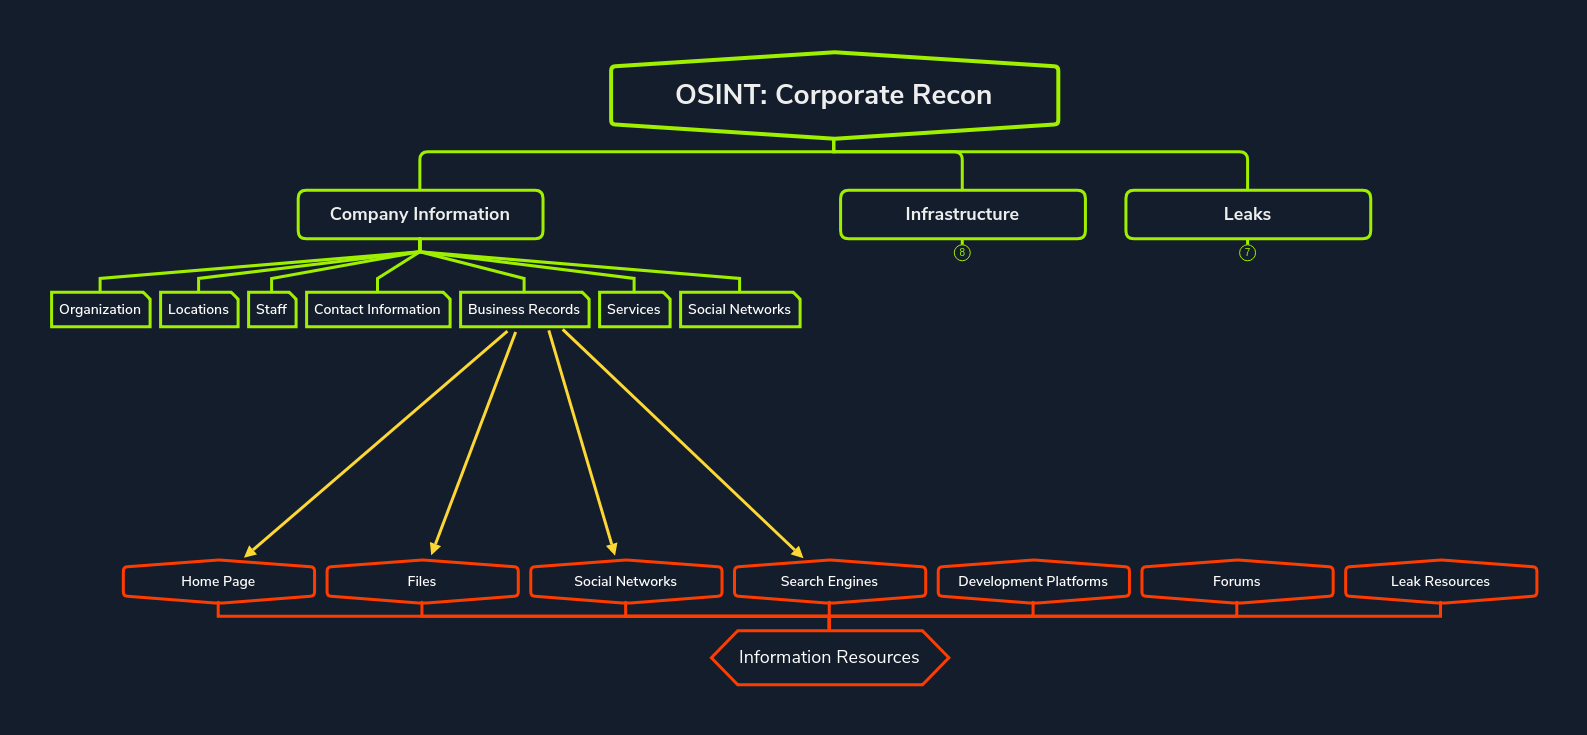
\includegraphics[width=\linewidth]{recon/osint/images/osint-business-records.png}
  \caption{OSINT Business records}
  \label{fig:osint-business-records}
\end{figure}

\subsubsection{Home Page}

{\bf Financial records} can give us a good overview of how the company is doing
and how it is currently growing. It also gives us information about what the
company depends on and whether it is presently healthy from a financial
standpoint. As soon as a company is under high pressure, it naturally tries to
save as much money as possible. These types of financial constraints often
force companies to seek out lower-quality services from third parties. It does
not matter whether these services are technical or not. With lower quality
services, it is more likely that they do not meet the highest security
standards and that we will be able to find some information about our target
company.

\subsubsection{Files}

Files that we can find on the internet contain not only potentially important
metadata but also general information. Every company must present itself
efficiently and profitably. After all, they want to attract new customers and
show their success to convince them to give them their business. Many companies
demonstrate their success through financial reports. These can be found on the
company's website or are sent to subscribers via newsletters.


Using Google search, we can find and filter out files like .docx, PDFs, and
others. We can use Google Dorks for these purposes. A small list of the most
important "dorks" can be found
\href{https://securitytrails.com/blog/google-hacking-techniques}{here}.

\subsubsection{Social Networks}

In addition to finances, the company's culture also plays an essential role.
This enables us to determine how certain situations are handled and how
reliably the processes function. Suppose a 3rd-level support staff member is
neglected and frustrated with their company's management concerning their
position. In that case, it is a very strong demotivator that consequently
reflects on their performance, attention, and attentiveness. This employee will
most likely put in far less effort and even less thought into the company's
future.

With the help of Google, we can find more reviews and reports about the
company. This will help us identify where the most difficulties and problems
occur in their processes that we can focus on later. It is essential to note
the perspective from which the reviews have been written. They can be written
either by customer or an employee. When we Google the reviews, we will find
sources such as Indeed.com, which gives us an excellent opportunity to look at
the reviews to get a better idea of the atmosphere and process.


\subsubsection{Search Engines}

On \href{https://www.crunchbase.com/}{Crunchbase.com}, we can find some of the
published records concerning our target company. Often we can find financial
reports from which we can find more helpful information. These reports also
list some information about employees.


If our customer is a publicly-traded corporation, it is even easier for us to
track its financial status. This is because we can view detailed information on
them on \href{https://finance.yahoo.com/}{Yahoo! Finance}.


For us as penetration testers, it is enormously important to look behind the
scenes and think outside the box. We need to understand how the company's
financial situation has developed and which data and factors have contributed
to this. If we know these, we can start to trace their management processes and
go into more detail to understand what steps were necessary and how we as
"attackers" could influence them by penetrating the corporate network.

\subsection{Services}
{\bf Services} are also explained in great detail on the website so that the
number of external inquiries is kept to a minimum. For this reason, how each
service is carried out is usually discussed in detail. All other questions that
arise are generally specific.

\begin{figure}
  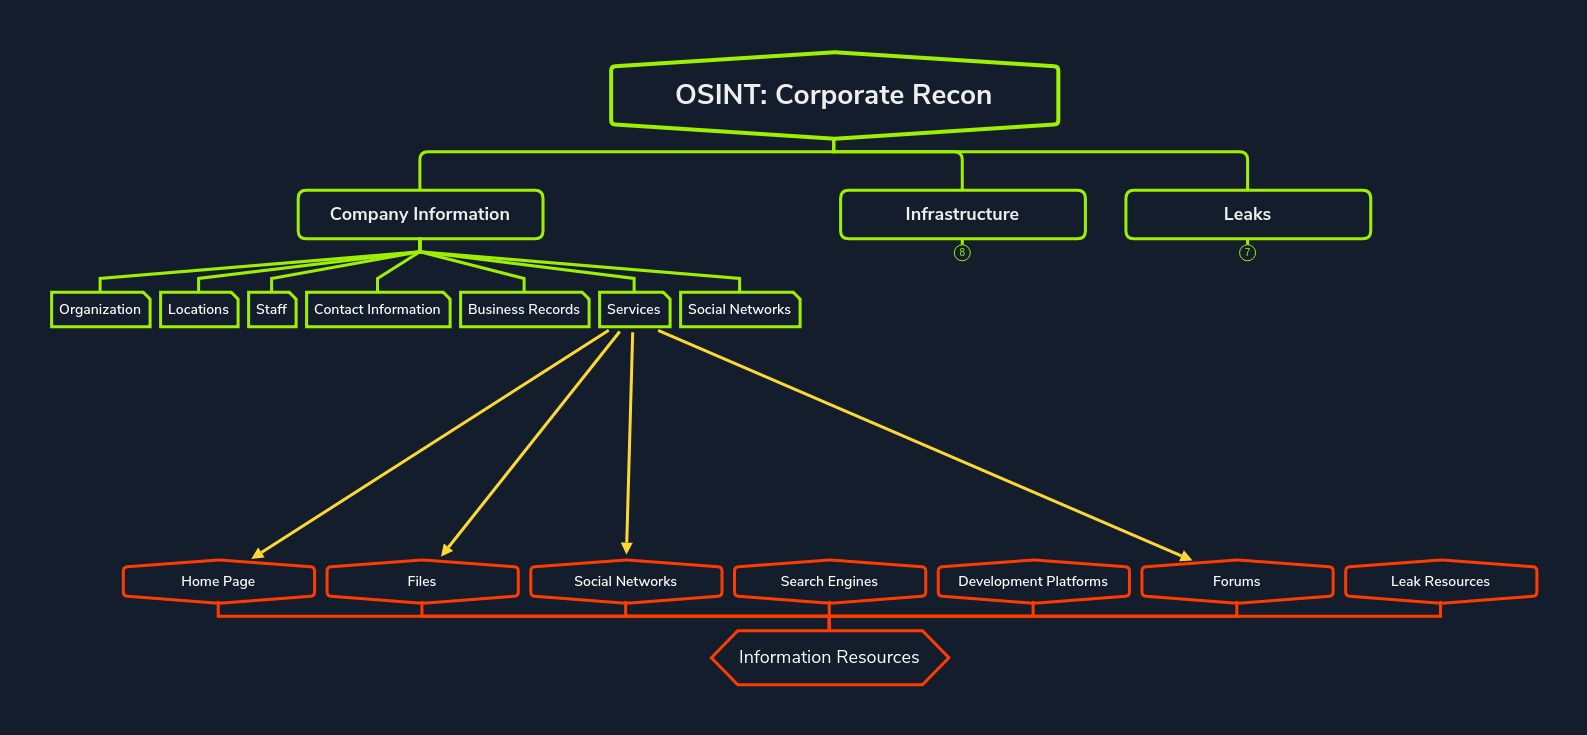
\includegraphics[width=\linewidth]{recon/osint/images/osint-services.png}
  \caption{OSINT Services}
  \label{fig:osint-services}
\end{figure}

\subsubsection{Home page}
On the product and service descriptions page, we will often find step-by-step
instructions that describe the entire process between the customer and the
completion of the service or the receipt of the product. Utilizing options that
are sometimes provided, such as the localization of the representative offices
and contact persons, we can also find, among other things, tools that the
website visitor can use.

These services may include information about the {\bf technologies}, their {\bf
workflow}, {\bf employees} who take care of these services, and resources that
may contain potentially security-sensitive information.

Suppose we are not familiar with the industry but want to find out how these
processes and orders are set up and managed. In that case, we should search
through the internet to find out what options are available and look at {\bf
similar providers} who may provide additional information. We must remember
that all companies in the same industry are usually competitors. At the same
time, the desire to be the \verb+#1+ in the marketplace brings the same desire to
provide the {\bf best possible services} to customers, which are often {\bf
very similar}. In many cases, the company also takes advantage of {\bf service
gaps} that the competitors do not or only poorly fulfill.

These are then often prioritized. This service is presented with much more information to show that this company is significantly better than the competition.

Nowadays, the management of services is done almost exclusively through a form
of software application. A high focus is placed on web applications and mobile
applications, making operation and control as easy as possible for customers.

\subsubsection{Files}

Information about the target company's {\bf partners} can also be found {\bf in
files}. This is because not all partners and technologies are presented and
disclosed directly. However, these companies may be marked as "{\bf Powered
by}" in these files.

As mentioned earlier, we can already see that our target company uses {\bf
cloud solutions} offered by the provider. This is also very valuable to us, as
we now know that we should be on the lookout for potential cloud-based storage
locations that may be publicly accessible.

\subsubsection{Social Networks}

In principle, social networks are used by companies for marketing purposes to
bring their products and services to the people and to draw attention to
themselves. Here, too, information about their services and solutions is
presented and published. In most cases, this is also linked so that these
solutions can be viewed directly and the company's website is visited. This can
play an essential role, especially with new releases of service solutions and
applications. If this has been tested poorly (or even not at all) for security
and vulnerabilities, then this application/solution represents a potential
attack vector.

\subsubsection{Forums}

A wide variety of technical discussions and news are discussed in forums. These
are very useful for us when we want to find out something about a company's
performance and services. Every post in the forum usually has a date when we
find out when an enhancement or application, or service was released. Based on
this time-lapse, we can roughly estimate how up-to-date specific software may
be. For example, if we find an application that uses a library containing a
vulnerability, we will be able to exploit it with the appropriate preparations
and measures. More information about vulnerable libraries and how many
applications are affected by those can be found in this
\href{https://www.veracode.com/blog/research/announcing-our-state-software-security-open-source-edition-report}{Veracode
report}.

Larger companies that have a large number of customers sometimes even provide
forums for customers. We can often register and peruse these forums. {\bf
Technical problems} are usually discussed there, and we can also ask questions
to find out more information. We can sometimes even see how the developers or
administrators solve specific problems. With a little bit of advanced
programming knowledge, we could even understand how a specific software-related
problem could be solved.




\subsection{Social Networks}
We can also ask where to find more information about the company during a phone
call. We are usually directed to {\bf blog posts}, {\bf videos}, or {\bf
documentation} from a marketing perspective that would give us better insight
into the company. We can find a variety of information about the target company
through the different social media networks. We usually first direct our focus
to the company's linked accounts via its home page. In turn, these may lead us
to different sources of information not mentioned on the home page.

We can also search the different platforms themselves to see where the company
is represented on social networks. Finally, we can use search engines or forums
to find out if the company is mentioned there.

\begin{figure}
  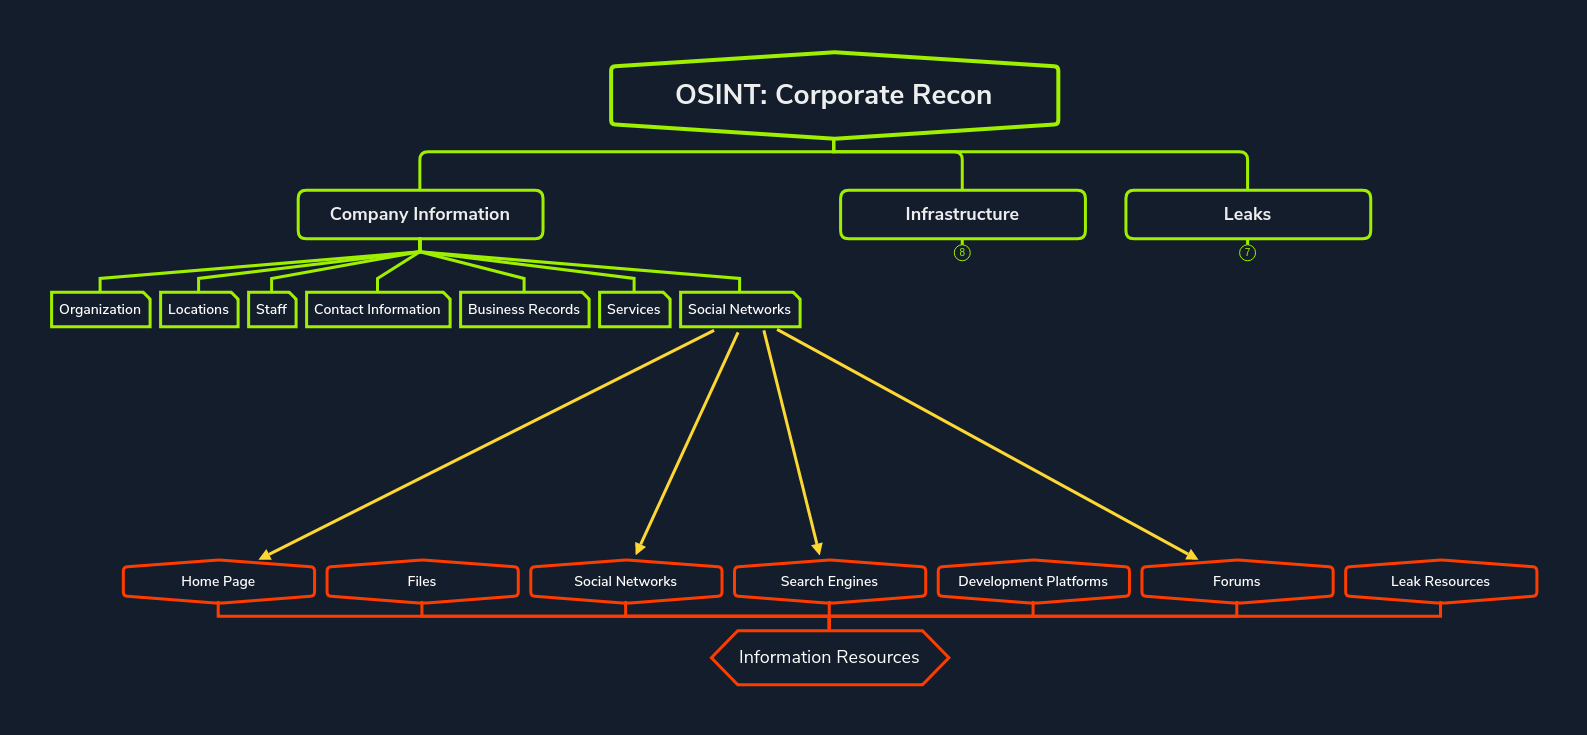
\includegraphics[width=\linewidth]{recon/osint/images/osint-social.png}
  \caption{OSINT Social}
  \label{fig:osint-social}
\end{figure}

With social networks, things can now get a bit more complicated and confusing,
as they serve as both information elements and sources of information. If we
look at social networks as sources of information, we enter what is known as
{\bf Social Media Intelligence (SOCMINT)}. To not lose the orientation and
overview of this, during the OSINT phase, we focus on the "movement" and
presence of the company's social networks. Therefore, in this case, we will
deal with the social networks and information elements. Once we get an overview
of the company's presence on the social networks, we can move into SOCMINT and
examine and analyze each platform in more detail.

To make the distinction clearer, we use social networks as Information Elements
(marked green) rather than Information Sources (marked red) in this phase. This
means that we are collecting the company's connections to social networks.

However, this does not mean that we have to limit ourselves here. We can combine both, but we have to keep in mind that we consider social networks as information elements (i.e., pure information for the company's value). We can find a lot of information about the company itself and its technologies. These include public and internal information but is not limited to:
\begin{verbatim}
Blogs/News 	Images & Videos 	Wikis 	Documents & Files 	Social Media
\end{verbatim}

\subsubsection{Home page}
Almost every medium-sized company strives to keep current and potential
customers up to date. In most cases, these sources are also straightforward to
find. After all, this news, which is also often published on blogs and social
media platforms, provides information about our target companies' progress and
success. This information is often provided to convince potential customers
that the company is always the best choice.

This news often includes new cooperations with partners and successes achieved
by the company. Additionally, new technologies and solutions for customers are
presented here that we should also consider. Soon we will look at a document
that may contain this type of information.

\subsubsection{Social Networks as Information Component}

Most companies see social media platforms as essential and indispensable from a
marketing point of view. In most cases, we find the links to the various
platforms directly on the website itself. On these social media platforms, such
as Twitter, LinkedIn, Xing, Facebook, Instagram, YouTube, and others, we find
not only the {\bf latest news} and {\bf developments} of the company but also
older posts that can give us information about the {\bf structure and
technologies}.

Another often overlooked component, which does not directly belong to the
social media category but fulfills the same purpose, is {\bf newsletters}.

\subsubsection{Search Engines}

All search engines also allow us to search for images and videos of the
company, which can also provide us with links to social networks and
information sources.

Companies often use {\bf images} and {\bf videos} to increase the
attractiveness of blog posts and news articles. In the last section, we have
already seen that we could identify a mobile application from a video and get a
short impression of how it looks. Now let's look at a picture of our target
company that provides us with some information.

i{\bf Photos} offer a far more significant security risk than most people
realize. Let us say we find a high-resolution photo of a company meeting where
the work {\bf IDs} are visible. Especially for {\bf red-team operations}, this
is incredibly beneficial because we can use the photo to recreate and prepare a
badge to get past the building's security personnel and get inside the
company's building.

The search for documents in this section is based on the fact that it allows us, among other things, to refer to sources on which social media platforms these files are stored.

A good start for finding documents and connections is Google. Using {\bf Google
Dorks}, we can define parameters that should be displayed. For this part, it is
enough to know that we can use the Google Dork "{\bf filetype:}" to define the
filetype that we are seeking. This results in output to links that explicitly
point to the specified file type of our target. Accordingly, we can download
and view them.

Do not forget that we must document each step and the corresponding source we
use to find the information. Otherwise, we will have difficulty describing how
and where we got this information from in the report.


Of course, we can and must also use other file types here. We will see later in
the section {\bf Internal Leaks} the valuable information these files can give
us, which can play a crucial role in the success of our engagement.

\subsubsection{Forums}
As mentioned earlier, forums serve as a good source of information for
technical difficulties and problems. Problems are also discussed and dealt with
on social networks. There are countless public forums such as Reddit,
StackOverflow, and others that the company can use for this purpose. Here, too,
we focus mainly on the presence of forums where people discuss our target
company.

Internal forums that we may stumble upon are very interesting to us. In these,
technical questions are answered in far greater detail than in public forums.
Therefore, we should keep an eye out if we can perhaps register on an internal
forum to search for information.

\subsubsection{Wikis}

The exciting thing about wikis is the information that is published and the
{\bf references} and {\bf external links}, which in turn point us to other
sources that can provide us with even more information. Some references and
resources can be Wikipedia, Github, or even {\bf internal/provided wikis} to
which it can be linked.

We can find a lot of helpful information from the wikis that describes the
company itself or its services. Wikis are created to provide detailed
information about specific topics and make them accessible to others. In other
words, they often serve as documentation that can provide valuable information
for us.

For example, we may find a post describing a specific application in detail
(i.e., how to install it, how to work with it, and more. We can determine which
    dependencies these applications have and can later use this information for
    Reverse Engineering to understand the developer better and uncover
    potential weaknesses.
